\chapter{System Concept}\label{chap:concept}
The following chapter will cover the system concept, the functionality it offers and the general functional system description. Also, the following sections should clarify how the SmartNotes application can be used, illustrate its design using the UML diagrams and prepare the reader for more detailed system description included in the chapter~\ref{chap:sys_description}.

The idea of SmartNotes has been inspired by the Google Notebook application which was being actively developed until January 2009, when Google announced that further development work on this project is stopped. Google Notebook has an interesting interface and features, some of them already motioned in section~\ref{subsec:google_notebook}. what was still missing from the functionality until January 2009 was comfortable notes usage without network connectivity. The aim of the subject of the thesis was to use the idea of making a truly scalable notes taking application that would be even more flexible.

\section{Functionality description}\label{sec:functionality_descr} 
Detailed description of how a system may be used should by of utmost importance both to the developer and to the end user, as it helps gain a general perspective, called 10,000-foot view\cite[page 49]{uml_use_case}, of the system and make useful observations. The implementation as well as the conceptual and system design decisions become a side issue, as the foreground is always occupied by the functionality  the application is to offer. For that reason, the use of case scenarios and flow charts will be very helpful in describing the efficient way of using the SmartNotes application.

Users willing to work on their notes disregarding network connectivity will need to install iSmartNotes, which is a graphical interface of SmartNotes. Specifically, the SmartNotes application is divided into the web-based system and the graphical desktop interface, a separation with which UI experiments can be done without the need of having the web browser open in order to work on the notes. The web based part of SmartNotes makes the synchronization feature possible and allows to monitor the entire system of SmartNotes. However, in order to use the synchronization feature, the iSmartNotes needs to be activated by the user. Additionally, since users of SmartNotes are expected to have a Google account\footnote{Creating a Google account by visiting \url{https://www.google.com/accounts/} gives a access to various services offered by the Google company where Gmail, Google News or Google Finance are one of the most popular tools. These are regarded secure and solid services users can relay on.} the activation code will be available after logging in to the SmartNotes system with that account. This process is illustrated on figure~\ref{fig:ismartnotes_activation}. The idea behind it is to make the use of the popular Google Account and not multiply the accounts to services that the user has to know the login and password. Basing on the activation key, the user is granted access to his personalized SmartNotes account and to the synchronization feature. Without the activation, iSmartNotes can be used as a regular notes editor.  
\begin{figure}[ht]
\begin{center}
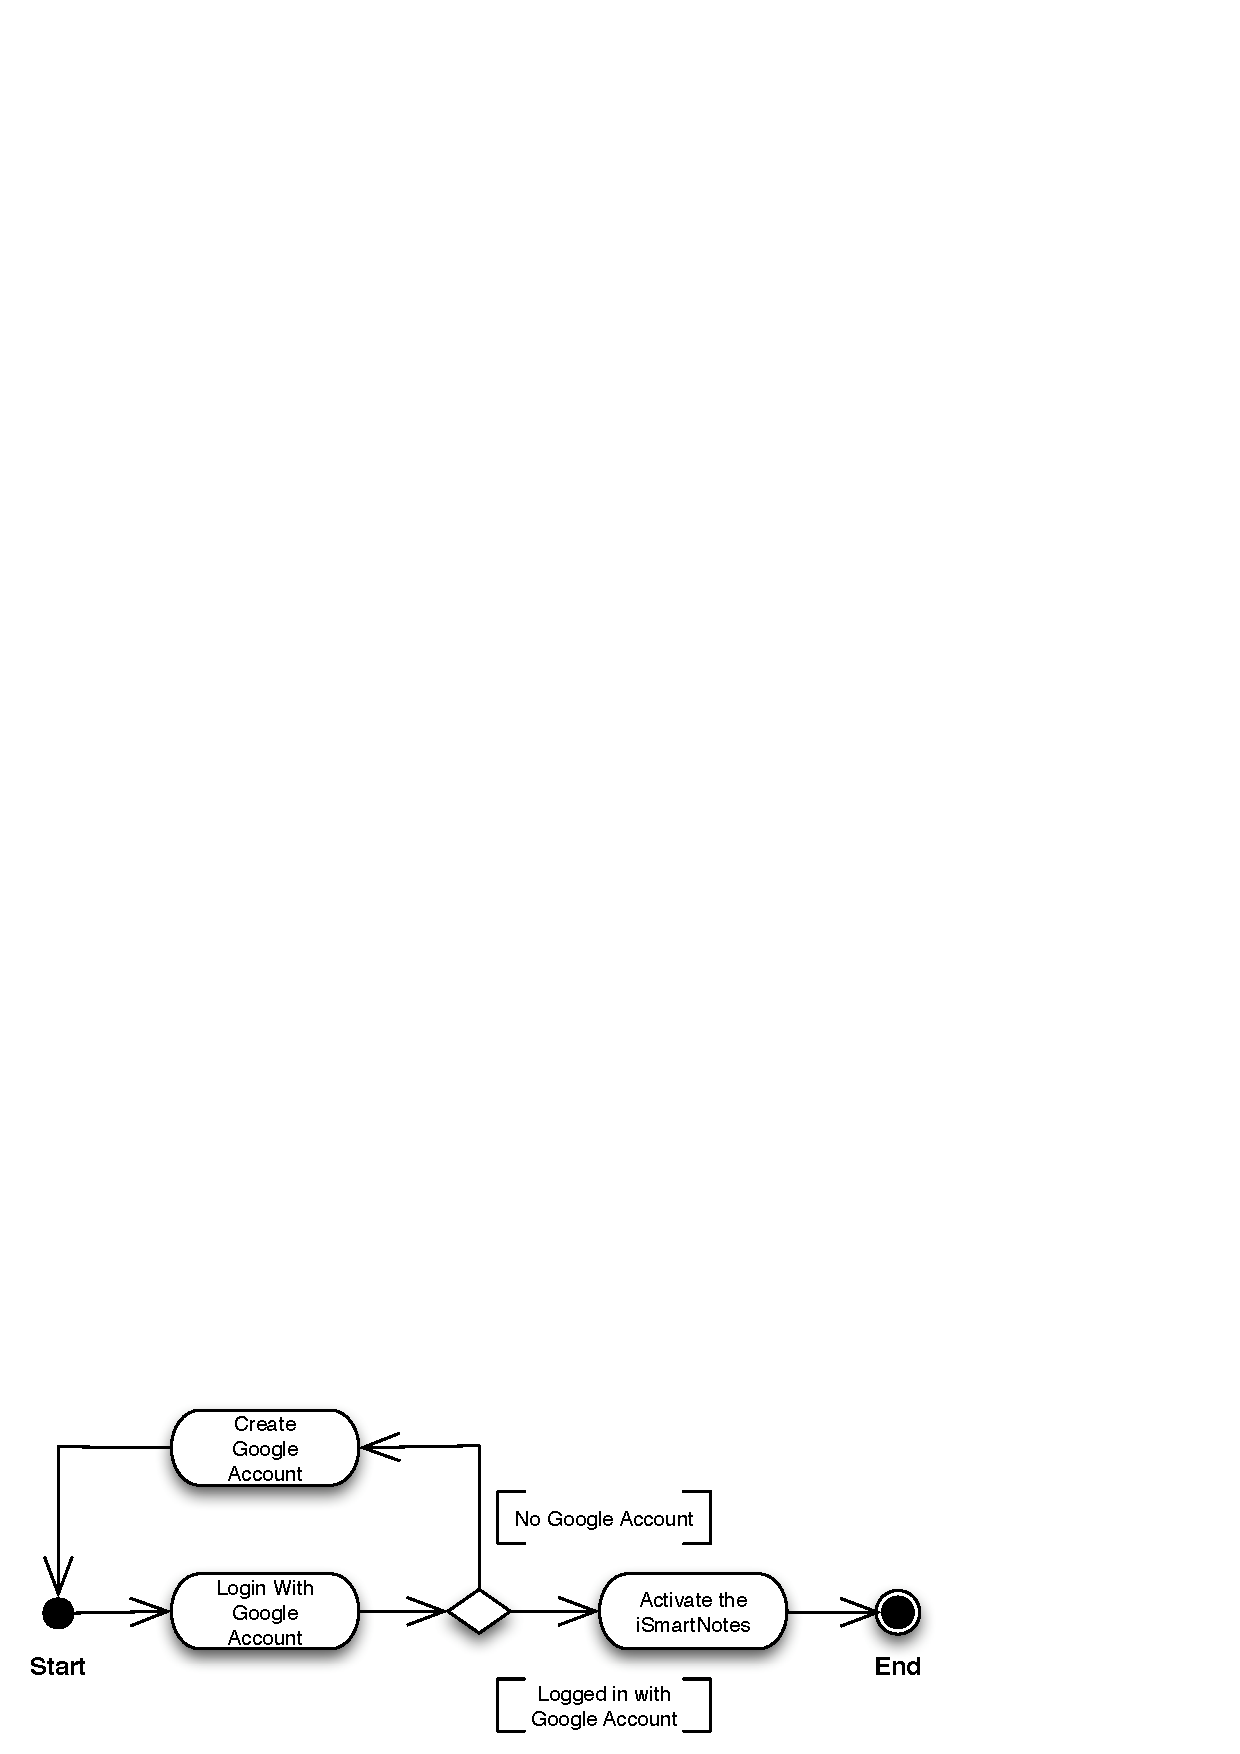
\includegraphics[scale=0.65]{charts/activate_iSmartNotes.png}
\caption{The iSmartNotes application activation with the Google Account.}
\label{fig:ismartnotes_activation}
\end{center}
\end{figure}
The skim of functionality offered by iSmartNotes is demonstrated on figure~\ref{fig:workon_ismartnotes}.
\begin{figure}[ht]
\begin{center}
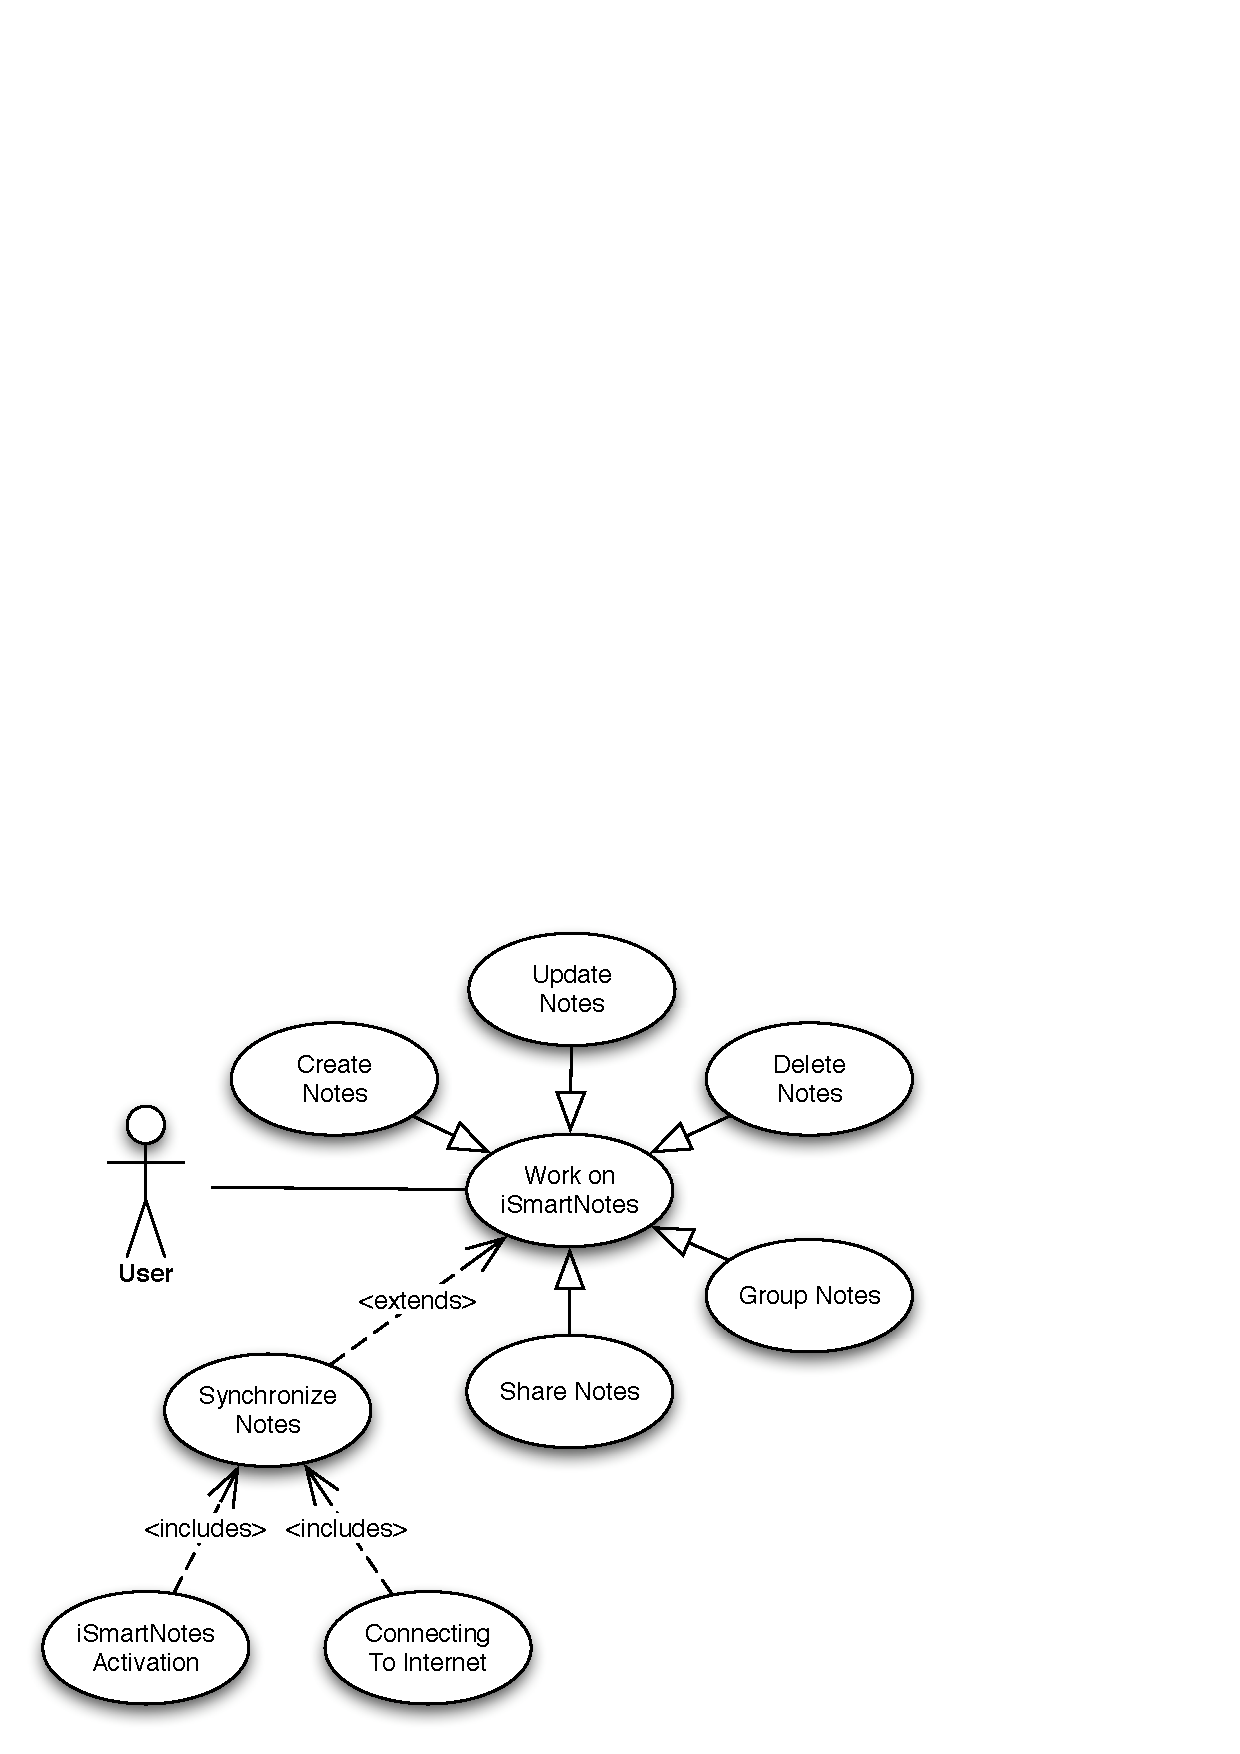
\includegraphics[scale=0.55]{charts/work_on_iSmartNotes.png}
\caption{The iSmartNotes application use cases.}
\label{fig:workon_ismartnotes}
\end{center}
\end{figure}
This includes the CRUD operations and three extra features. Firstly, the notes can be easily grouped together in named tabs, which should make organizing and finding notes much easier. Secondly, it is possible to publish the notes marked as shared. The final feature is the synchronization process that requires iSmartNotes activation and network connection to contact with the web-based part of SmartNotes. What remains to be discussed is the cooperation between iSmartNotes and the web-based part of SmartNotes, therefore, the relation between them and the functionality offered to the user and administrator are shown on figure~\ref{fig:ismartnotes_smartnotes}. 
\begin{figure}[ht]
\begin{center}
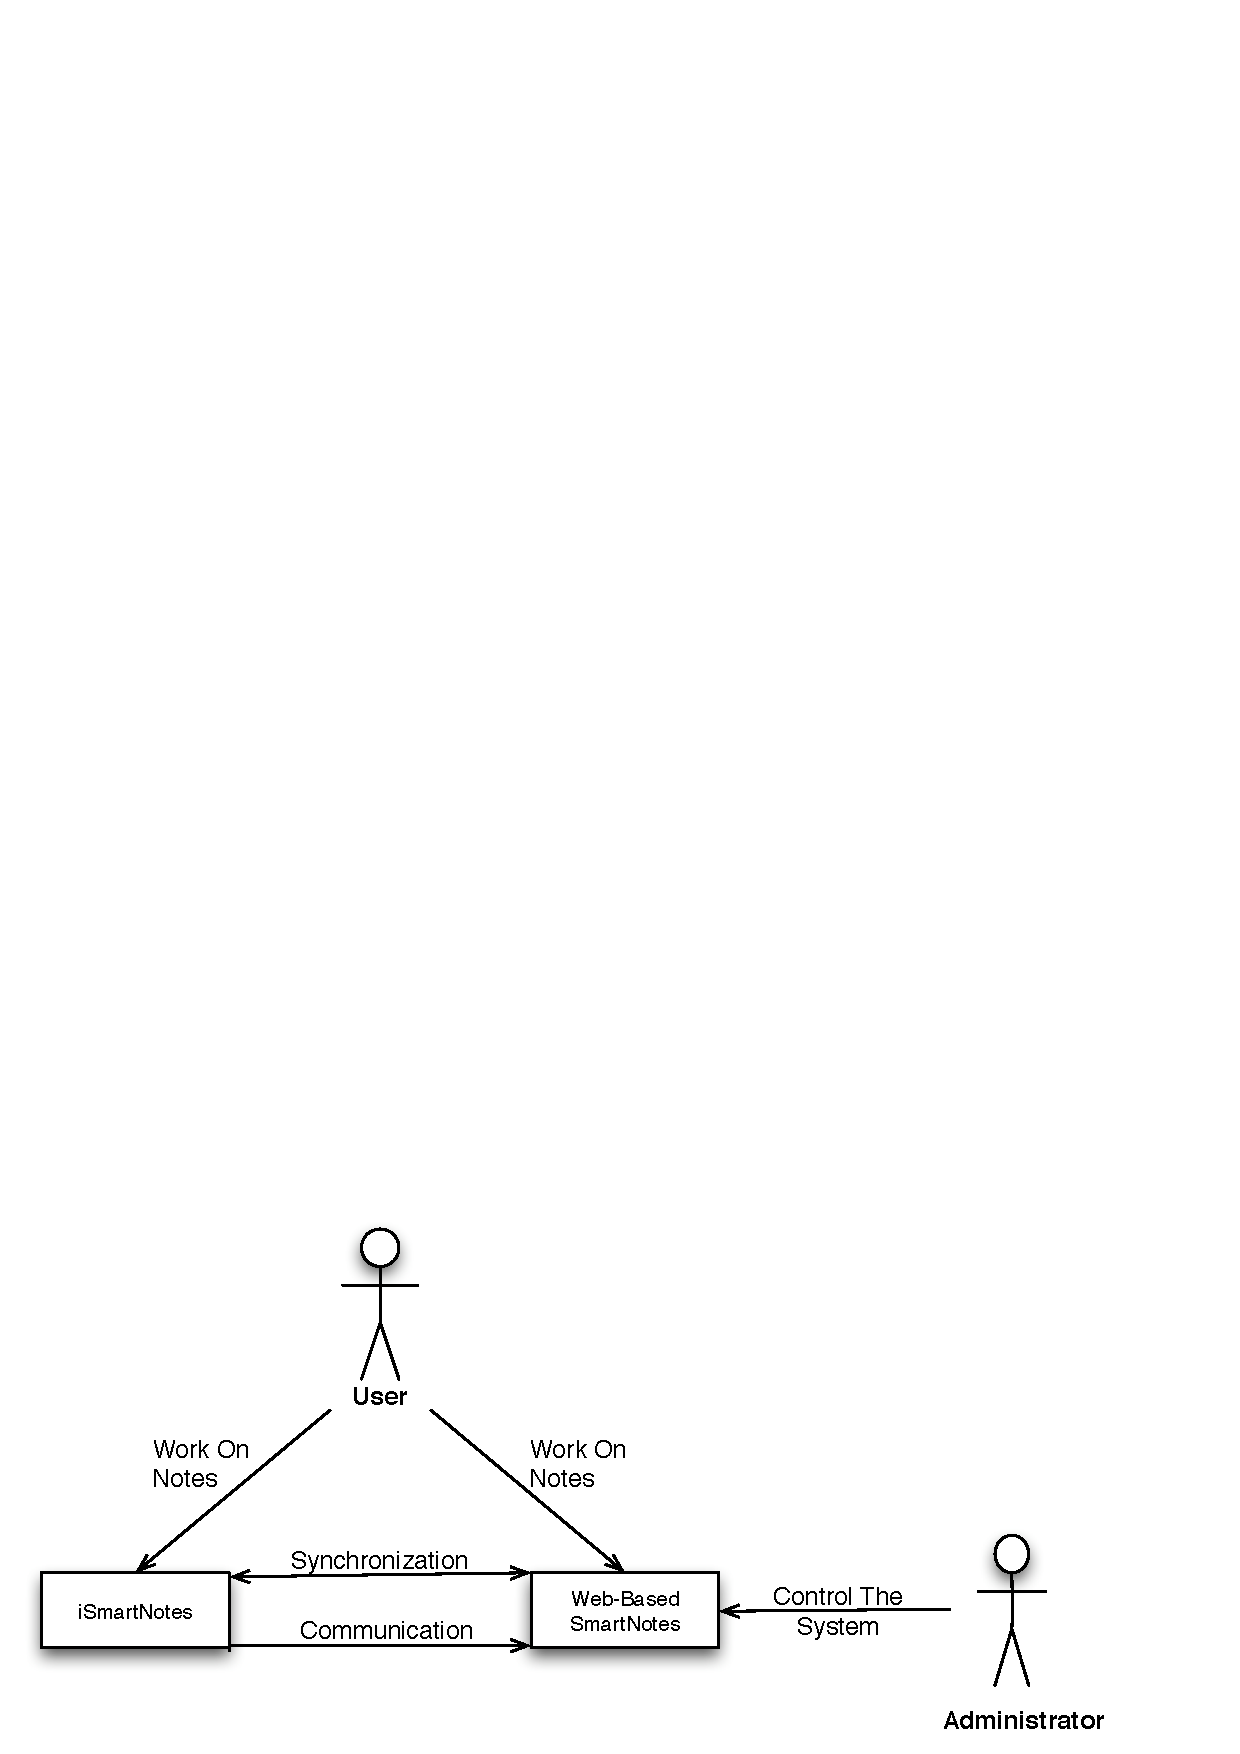
\includegraphics[scale=0.55]{charts/iSmartNotes_SmartNotes.png}
\caption{The cooperation of iSmartNotes and web based SmartNotes.}
\label{fig:ismartnotes_smartnotes}
\end{center}
\end{figure}

This interesting concept allows the user to work on iSmartNotes as well as the Web-based part of SmartNotes exchangeably, at the same time letting the SmartNotes application care for work synchronization, which has been also highlighted in the above discussed picture. Yet, however functional and elastic the application may seem, the same functionality is not feasible in the web interface of the present project, even if the administrator is granted access to tools like datastore data browser, system status or application dashboard described in section~\ref{sec:gae_general}. This can help to quickly diagnose faults within the application and rollback it to the latest stable version. Moreover,  it can indicate that the rescuers are not sufficient to serve the traffic and eventually extend them. The tools work effectively in cooperation with Google Webmaster Tools and the Google Analytics as they can provide more information concerning the web page and its visitors.

It appears to be worth describing the synchronization feature in more detail. The feature is realized by the VCS which was introduced in section~\ref{sec:popular_vcs}. No matter if the user works online or not, they have full access to notes and synchronize them online. As it has been marked on the graph from figure~\ref{fig:ismartnotes_smartnotes}, the synchronization process is bidirectional: it is triggered from the web-based part of SmartNotes, which plays a role of the main server, and the iSmartNotes, playnig the role of clients and reverse. This type of set-up should allow to update the notes whenever necessary. Another point presented in figure~\ref{fig:ismartnotes_smartnotes} is the directional communication between iSmartNotes and SmartNotes, which should be understand as an additional logic allowing to perform operations on the user side by the help of iSmartNotes, including the display of user information on significant events like availability of new features or versions.  As a matter of fact, the process is directional in one way as it is the iSmartNotes application which receives the information from the SmartNotes server and displays it to the user. Whereas the presented functionality does not fully exploit the possible feature list, as mentioned in section~\ref{subsec:vcs_comparison}, it is a good practice to keep the application as simple as possible and focus on a set of clearly defined key features.

\section{Functional description}\label{sec:functional_descr}
The SmartNotes application should run on a infrastructure that can ensure complete availability and high load. Easy system maintenance and openness to future expansion in functionality are also strongly desirable features. It is not pointless to mention that the above requires resource usage, which makes the financial model of utmost importance and is the already introduced 10,000-foot view of system requirements. Adding a friendly deployment methodology and good documentation is what would satisfy the most demanding developer.

Admittedly, in order for the application to gain popularity, users should be well informed about the application and its functionality; also, it is vital to provide availability of instructions on how to get started. For these reasons, the landing page should be not only informal and practical, but also international to reach greater group of users.

From the architectural point of view, SmartNotes is a simple client-server application, the only difference being the usage of DVCS, which allows the machines to access thesame set of commands and make their hard disks hold the entire repository with its history. Yet, it may be confusing that it still remains a client-server architecture, but just as the centralized VCS do not recognize any other architecture than the client server, the distributed VCS uses it as one of possible use cases. In the following scenario one of the machines fulfills a role of the reverential server to which all remaining machines direct their requests, at the same time being a for of public repository with the most recent version that should be always available to users. In consequence, each client requires the installation of DVCS as one of the main components, while the size of the chosen VCS matters as much as its performance, which all in all has significant impact on the final performance of iSmartNotes. For optimum user experience, the iSmartNotes application provides an easy-to-install package that could be downloaded from the server serving static content, which is not only a faster solution from dynamically served content, but also allows to save system resources, costing a minimum of CPU time.

The next two sections state certain problems related to synchronization scenarios using VCS and the application activation. They will be analyzed focusing on the evaluating of a number of possible solutions and the argumentation will lead to the choice of the most optimal solution.  
 
\subsection{Synchronization scenarios using version control systems}\label{subsec:sync_scenarios}
It is one of the roles of VCS to keep the repositories updated, nevertheless, they never perform it without a user request\footnote{This means that the user has to run an appropriate command or click on the right button when using a graphical interface. It could be naturally automated by writing a script that would perform that task for the user or by setting a cron job with a desired time interval, but the tool still requires the user to trigger the update process.}, the reasons for which are various, but dealing with conflict situations like the one shown on figure~\ref{fig:google_notebook} seems to be the most important one. To put this in simple words, it is a situation when the VCS needs the user decision to resolve the conflict situation. In such case, the way the merging is performed also differs in numerous VCSs, yet from the user perspective, operations like update and merge are easy to imagine, basing on the final result. 

Fetch implemented by git system consists of three steps:
\begin{enumerate}
\item{lookup}
\item{getting changes}
\item{updating or merging}
\end{enumerate}
\subsection{iSmartNotes activation process}\label{subsec:ismartnotes_activation}
